% Options for packages loaded elsewhere
\PassOptionsToPackage{unicode}{hyperref}
\PassOptionsToPackage{hyphens}{url}
\PassOptionsToPackage{dvipsnames,svgnames,x11names}{xcolor}
%
\documentclass[
  letterpaper,
  DIV=11,
  numbers=noendperiod]{scrreprt}

\usepackage{amsmath,amssymb}
\usepackage{lmodern}
\usepackage{iftex}
\ifPDFTeX
  \usepackage[T1]{fontenc}
  \usepackage[utf8]{inputenc}
  \usepackage{textcomp} % provide euro and other symbols
\else % if luatex or xetex
  \usepackage{unicode-math}
  \defaultfontfeatures{Scale=MatchLowercase}
  \defaultfontfeatures[\rmfamily]{Ligatures=TeX,Scale=1}
\fi
% Use upquote if available, for straight quotes in verbatim environments
\IfFileExists{upquote.sty}{\usepackage{upquote}}{}
\IfFileExists{microtype.sty}{% use microtype if available
  \usepackage[]{microtype}
  \UseMicrotypeSet[protrusion]{basicmath} % disable protrusion for tt fonts
}{}
\makeatletter
\@ifundefined{KOMAClassName}{% if non-KOMA class
  \IfFileExists{parskip.sty}{%
    \usepackage{parskip}
  }{% else
    \setlength{\parindent}{0pt}
    \setlength{\parskip}{6pt plus 2pt minus 1pt}}
}{% if KOMA class
  \KOMAoptions{parskip=half}}
\makeatother
\usepackage{xcolor}
\setlength{\emergencystretch}{3em} % prevent overfull lines
\setcounter{secnumdepth}{5}
% Make \paragraph and \subparagraph free-standing
\ifx\paragraph\undefined\else
  \let\oldparagraph\paragraph
  \renewcommand{\paragraph}[1]{\oldparagraph{#1}\mbox{}}
\fi
\ifx\subparagraph\undefined\else
  \let\oldsubparagraph\subparagraph
  \renewcommand{\subparagraph}[1]{\oldsubparagraph{#1}\mbox{}}
\fi

\usepackage{color}
\usepackage{fancyvrb}
\newcommand{\VerbBar}{|}
\newcommand{\VERB}{\Verb[commandchars=\\\{\}]}
\DefineVerbatimEnvironment{Highlighting}{Verbatim}{commandchars=\\\{\}}
% Add ',fontsize=\small' for more characters per line
\usepackage{framed}
\definecolor{shadecolor}{RGB}{241,243,245}
\newenvironment{Shaded}{\begin{snugshade}}{\end{snugshade}}
\newcommand{\AlertTok}[1]{\textcolor[rgb]{0.68,0.00,0.00}{#1}}
\newcommand{\AnnotationTok}[1]{\textcolor[rgb]{0.37,0.37,0.37}{#1}}
\newcommand{\AttributeTok}[1]{\textcolor[rgb]{0.40,0.45,0.13}{#1}}
\newcommand{\BaseNTok}[1]{\textcolor[rgb]{0.68,0.00,0.00}{#1}}
\newcommand{\BuiltInTok}[1]{\textcolor[rgb]{0.00,0.23,0.31}{#1}}
\newcommand{\CharTok}[1]{\textcolor[rgb]{0.13,0.47,0.30}{#1}}
\newcommand{\CommentTok}[1]{\textcolor[rgb]{0.37,0.37,0.37}{#1}}
\newcommand{\CommentVarTok}[1]{\textcolor[rgb]{0.37,0.37,0.37}{\textit{#1}}}
\newcommand{\ConstantTok}[1]{\textcolor[rgb]{0.56,0.35,0.01}{#1}}
\newcommand{\ControlFlowTok}[1]{\textcolor[rgb]{0.00,0.23,0.31}{#1}}
\newcommand{\DataTypeTok}[1]{\textcolor[rgb]{0.68,0.00,0.00}{#1}}
\newcommand{\DecValTok}[1]{\textcolor[rgb]{0.68,0.00,0.00}{#1}}
\newcommand{\DocumentationTok}[1]{\textcolor[rgb]{0.37,0.37,0.37}{\textit{#1}}}
\newcommand{\ErrorTok}[1]{\textcolor[rgb]{0.68,0.00,0.00}{#1}}
\newcommand{\ExtensionTok}[1]{\textcolor[rgb]{0.00,0.23,0.31}{#1}}
\newcommand{\FloatTok}[1]{\textcolor[rgb]{0.68,0.00,0.00}{#1}}
\newcommand{\FunctionTok}[1]{\textcolor[rgb]{0.28,0.35,0.67}{#1}}
\newcommand{\ImportTok}[1]{\textcolor[rgb]{0.00,0.46,0.62}{#1}}
\newcommand{\InformationTok}[1]{\textcolor[rgb]{0.37,0.37,0.37}{#1}}
\newcommand{\KeywordTok}[1]{\textcolor[rgb]{0.00,0.23,0.31}{#1}}
\newcommand{\NormalTok}[1]{\textcolor[rgb]{0.00,0.23,0.31}{#1}}
\newcommand{\OperatorTok}[1]{\textcolor[rgb]{0.37,0.37,0.37}{#1}}
\newcommand{\OtherTok}[1]{\textcolor[rgb]{0.00,0.23,0.31}{#1}}
\newcommand{\PreprocessorTok}[1]{\textcolor[rgb]{0.68,0.00,0.00}{#1}}
\newcommand{\RegionMarkerTok}[1]{\textcolor[rgb]{0.00,0.23,0.31}{#1}}
\newcommand{\SpecialCharTok}[1]{\textcolor[rgb]{0.37,0.37,0.37}{#1}}
\newcommand{\SpecialStringTok}[1]{\textcolor[rgb]{0.13,0.47,0.30}{#1}}
\newcommand{\StringTok}[1]{\textcolor[rgb]{0.13,0.47,0.30}{#1}}
\newcommand{\VariableTok}[1]{\textcolor[rgb]{0.07,0.07,0.07}{#1}}
\newcommand{\VerbatimStringTok}[1]{\textcolor[rgb]{0.13,0.47,0.30}{#1}}
\newcommand{\WarningTok}[1]{\textcolor[rgb]{0.37,0.37,0.37}{\textit{#1}}}

\providecommand{\tightlist}{%
  \setlength{\itemsep}{0pt}\setlength{\parskip}{0pt}}\usepackage{longtable,booktabs,array}
\usepackage{calc} % for calculating minipage widths
% Correct order of tables after \paragraph or \subparagraph
\usepackage{etoolbox}
\makeatletter
\patchcmd\longtable{\par}{\if@noskipsec\mbox{}\fi\par}{}{}
\makeatother
% Allow footnotes in longtable head/foot
\IfFileExists{footnotehyper.sty}{\usepackage{footnotehyper}}{\usepackage{footnote}}
\makesavenoteenv{longtable}
\usepackage{graphicx}
\makeatletter
\def\maxwidth{\ifdim\Gin@nat@width>\linewidth\linewidth\else\Gin@nat@width\fi}
\def\maxheight{\ifdim\Gin@nat@height>\textheight\textheight\else\Gin@nat@height\fi}
\makeatother
% Scale images if necessary, so that they will not overflow the page
% margins by default, and it is still possible to overwrite the defaults
% using explicit options in \includegraphics[width, height, ...]{}
\setkeys{Gin}{width=\maxwidth,height=\maxheight,keepaspectratio}
% Set default figure placement to htbp
\makeatletter
\def\fps@figure{htbp}
\makeatother

\KOMAoption{captions}{tableheading}
\makeatletter
\makeatother
\makeatletter
\@ifpackageloaded{bookmark}{}{\usepackage{bookmark}}
\makeatother
\makeatletter
\@ifpackageloaded{caption}{}{\usepackage{caption}}
\AtBeginDocument{%
\ifdefined\contentsname
  \renewcommand*\contentsname{Table of contents}
\else
  \newcommand\contentsname{Table of contents}
\fi
\ifdefined\listfigurename
  \renewcommand*\listfigurename{List of Figures}
\else
  \newcommand\listfigurename{List of Figures}
\fi
\ifdefined\listtablename
  \renewcommand*\listtablename{List of Tables}
\else
  \newcommand\listtablename{List of Tables}
\fi
\ifdefined\figurename
  \renewcommand*\figurename{Figure}
\else
  \newcommand\figurename{Figure}
\fi
\ifdefined\tablename
  \renewcommand*\tablename{Table}
\else
  \newcommand\tablename{Table}
\fi
}
\@ifpackageloaded{float}{}{\usepackage{float}}
\floatstyle{ruled}
\@ifundefined{c@chapter}{\newfloat{codelisting}{h}{lop}}{\newfloat{codelisting}{h}{lop}[chapter]}
\floatname{codelisting}{Listing}
\newcommand*\listoflistings{\listof{codelisting}{List of Listings}}
\makeatother
\makeatletter
\@ifpackageloaded{caption}{}{\usepackage{caption}}
\@ifpackageloaded{subcaption}{}{\usepackage{subcaption}}
\makeatother
\makeatletter
\@ifpackageloaded{tcolorbox}{}{\usepackage[many]{tcolorbox}}
\makeatother
\makeatletter
\@ifundefined{shadecolor}{\definecolor{shadecolor}{rgb}{.97, .97, .97}}
\makeatother
\makeatletter
\makeatother
\ifLuaTeX
  \usepackage{selnolig}  % disable illegal ligatures
\fi
\IfFileExists{bookmark.sty}{\usepackage{bookmark}}{\usepackage{hyperref}}
\IfFileExists{xurl.sty}{\usepackage{xurl}}{} % add URL line breaks if available
\urlstyle{same} % disable monospaced font for URLs
\hypersetup{
  pdftitle={SABRİ DEMİRDAL Progress Journal},
  colorlinks=true,
  linkcolor={blue},
  filecolor={Maroon},
  citecolor={Blue},
  urlcolor={Blue},
  pdfcreator={LaTeX via pandoc}}

\title{SABRİ DEMİRDAL Progress Journal}
\author{}
\date{}

\begin{document}
\maketitle
\ifdefined\Shaded\renewenvironment{Shaded}{\begin{tcolorbox}[interior hidden, frame hidden, enhanced, breakable, boxrule=0pt, borderline west={3pt}{0pt}{shadecolor}, sharp corners]}{\end{tcolorbox}}\fi

\renewcommand*\contentsname{Table of contents}
{
\hypersetup{linkcolor=}
\setcounter{tocdepth}{2}
\tableofcontents
}
\bookmarksetup{startatroot}

\hypertarget{introduction}{%
\chapter*{Introduction}\label{introduction}}
\addcontentsline{toc}{chapter}{Introduction}

This progress journal covers {[}STUDENT NAME SURNAME / PROJECT GROUP
NAME{]}'s work during their term at
\href{https://mef-bda503.github.io/fall22/}{BDA 503 Fall 2022}.

Each section is an assignment or an individual work.

\bookmarksetup{startatroot}

\hypertarget{about-myself}{%
\chapter{ABOUT MYSELF}\label{about-myself}}

title: '' Assignment 1'' author: ``Sabri Demirdal'' date: ``2023-01-02''

\begin{center}\rule{0.5\linewidth}{0.5pt}\end{center}

This is a template example qmd output page. You may see an example R
code below.

Firstly, I'm Sabri and I graduated from Bogazici university department
of economics in 2020. After the graduation, I started to work in the
investment office of the Presidency of Republic of Turkey and I have
been working here for almost two years as an Analyst.Even if I am
dealing with some data process like FDI report and some sector analysis
in Turkey in my job, I want to go deeper into data science and work in
the more sophisticated and technical job that related to in that
area.Therefore I started to Big Data Analytics master program at MEF
university.In this sense, despite the fact that until the university I
had no idea and any information about this area but some courses that I
took in the university and some online bootcamps in the coursera and
udemy like platforms bring my knowledge to some level, so with this
master program I hope to achive enough proficiency to start a good job
in this field.

You access my Linkedin account by clicking
\href{https://www.linkedin.com/in/sabri-demirdal-0508a1169/}{here},

and my \textbf{E-mail}
\href{mailto:sdemirdal@invest.gov.tr}{\nolinkurl{sdemirdal@invest.gov.tr}}

\bookmarksetup{startatroot}

\hypertarget{my-favorite-user-2022-video}{%
\chapter{MY FAVORITE UseR-2022
VİDEO}\label{my-favorite-user-2022-video}}

\hypertarget{wenxi-zhang---k-means-clustering-usage-in-datasets-with-missing-values}{%
\section{Wenxi Zhang - k-means clustering usage in datasets with missing
values}\label{wenxi-zhang---k-means-clustering-usage-in-datasets-with-missing-values}}

This content from Wenzi Zhang who graduated from Columbia University.
She aim to utilize a modified K-means algorithm to handle data with
missing values.

K-means clustering is a very popular type of unsupervised learning and
it is a clustering method that aims to partition n observations into k
clusters in which each observation belongs to the cluster with the
nearest cluster centroid and used commonly in machine learning models.

\begin{figure}

{\centering \includegraphics{https://static.javatpoint.com/tutorial/machine-learning/images/k-means-clustering-algorithm-in-machine-learning.png}

}

\caption{K means Clustering}

\end{figure}

However, the standard K-means algorithm fails to accomodate data with
missing values. This modified k-means algorithm below takes missing
values into account. When calculating the sum squared error of each data
point to the centroid, we only consider the partial distance with
entries with non-NA values. This innovation in the algorithm could be
beneficial for large sparse datasets with missing values, especially for
datasets of recommendation systems.

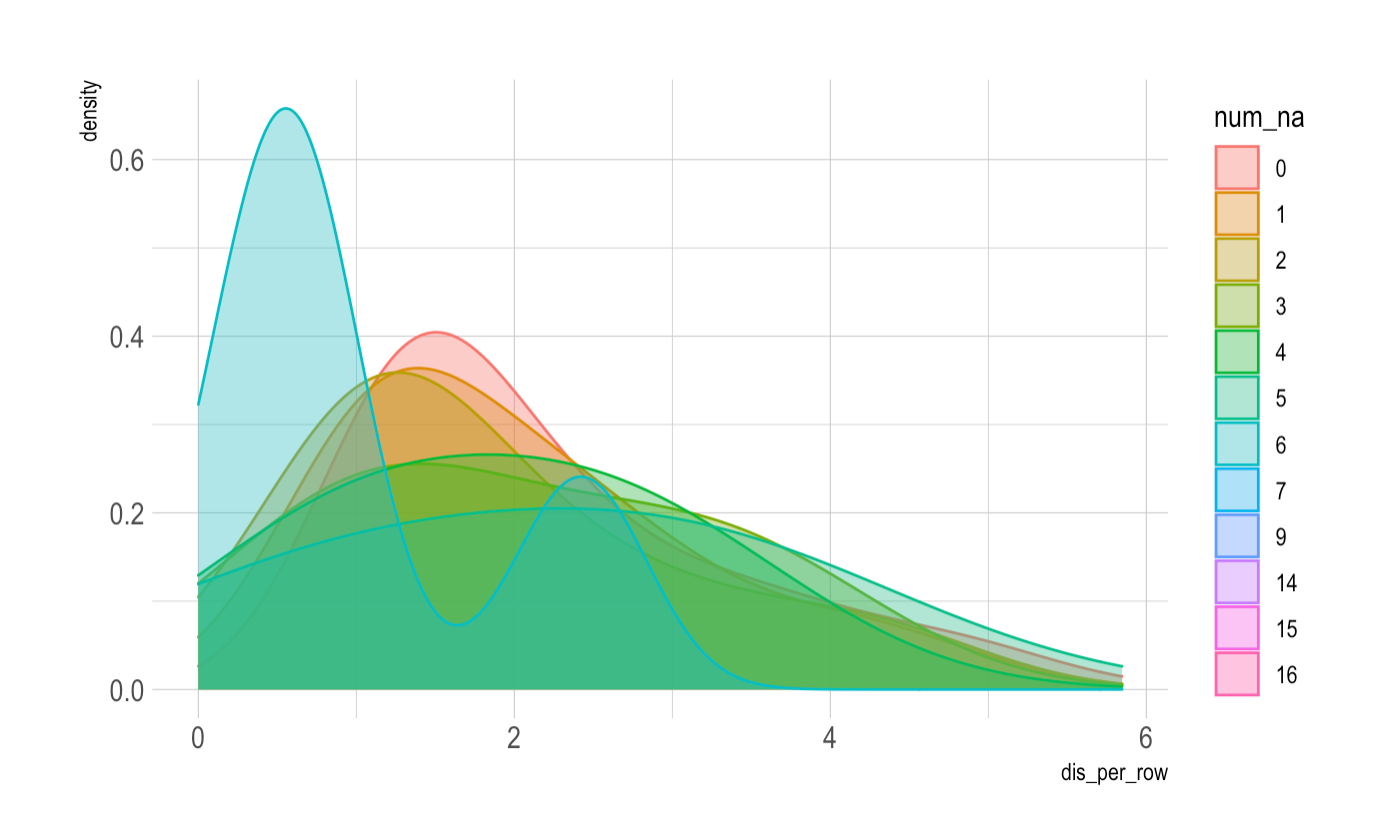
\includegraphics{./housevotes_density.png}\\

\bookmarksetup{startatroot}

\hypertarget{r-posts-relevant-my-interest}{%
\chapter{3 R POSTS RELEVANT MY
İNTEREST}\label{r-posts-relevant-my-interest}}

\hypertarget{downloading-data-using-quantmod-package-in-r}{%
\section{Downloading Data Using Quantmod Package in
R}\label{downloading-data-using-quantmod-package-in-r}}

Quantmod provides a very powerful function for downloading financial
data from the web. This function is called getSymbols. The getSymbols()
method sends a request to download and manage data from public sources
or local data. It is necessary to pass some parameters within this
method to make the desired request. The first argument of this function
is a character vector specifying the names of the symbols to be
downloaded. Then you can specify the source from which you want to get
the data.

The quantmod package is capable of downloading data from a variety of
sources. The current supported sources are: yahoo, google, MySQL, FRED,
csv, RData, and oanda. For example, FRED (Federal Reserve Economic
Data), is a database of 20,070 U.S. economic time series
(\includegraphics{http://research.stlouisfed.org/fred2/.pdf}).

\textbf{Example: USD/EUR exchange rates from Oanda}

\begin{Shaded}
\begin{Highlighting}[]
\FunctionTok{library}\NormalTok{(}\StringTok{\textquotesingle{}quantmod\textquotesingle{}}\NormalTok{)}
\end{Highlighting}
\end{Shaded}

\begin{verbatim}
Zorunlu paket yükleniyor: xts
\end{verbatim}

\begin{verbatim}
Zorunlu paket yükleniyor: zoo
\end{verbatim}

\begin{verbatim}

Attaching package: 'zoo'
\end{verbatim}

\begin{verbatim}
The following objects are masked from 'package:base':

    as.Date, as.Date.numeric
\end{verbatim}

\begin{verbatim}
Zorunlu paket yükleniyor: TTR
\end{verbatim}

\begin{verbatim}
Registered S3 method overwritten by 'quantmod':
  method            from
  as.zoo.data.frame zoo 
\end{verbatim}

\begin{Shaded}
\begin{Highlighting}[]
\FunctionTok{getSymbols}\NormalTok{(}\AttributeTok{Symbols =} \StringTok{\textquotesingle{}USD/EUR\textquotesingle{}}\NormalTok{, }\AttributeTok{src =} \StringTok{\textquotesingle{}oanda\textquotesingle{}}\NormalTok{)}
\end{Highlighting}
\end{Shaded}

\begin{verbatim}
[1] "USD/EUR"
\end{verbatim}

Here we have loaded the data for USD/EUR from the Oanda API which
provides free currency data. The getSymbols() method doesn't return any
output. Instead, it creates an internal object in the Global Environment
which in this case is the USDEUR object. The data object is an
``extensible time series'' (xts) object.

\begin{Shaded}
\begin{Highlighting}[]
\FunctionTok{head}\NormalTok{(USDEUR,}\DecValTok{15}\NormalTok{)}
\end{Highlighting}
\end{Shaded}

\begin{verbatim}
            USD.EUR
2022-07-07 0.982164
2022-07-08 0.984228
2022-07-09 0.981802
2022-07-10 0.981912
2022-07-11 0.990361
2022-07-12 0.996664
2022-07-13 0.995145
2022-07-14 0.998234
2022-07-15 0.994514
2022-07-16 0.991302
2022-07-17 0.991318
2022-07-18 0.986617
2022-07-19 0.979669
2022-07-20 0.979136
2022-07-21 0.980104
\end{verbatim}

To see the starting point of the data, type the following command. It
fetches and displays the first 15 rows of the data.

\href{https://financetrain.com/downloading-data-using-quantmod-package-in-r}{Here}
is the full post.

\hypertarget{the-power-of-mutate-for-data-wrangling-in-r}{%
\section{The Power of mutate( ) for Data Wrangling in
R}\label{the-power-of-mutate-for-data-wrangling-in-r}}

mutate() is a dplyr function that adds new variables and preserves
existing ones. That's what the documentation says. So when you want to
add new variables or change one already in the dataset, that's your good
ally. Given our dataset df , we can easily add columns with
calculations.

\begin{Shaded}
\begin{Highlighting}[]
\NormalTok{df }\OtherTok{\textless{}{-}} \FunctionTok{data.frame}\NormalTok{(}\AttributeTok{col1=}\FunctionTok{c}\NormalTok{(}\DecValTok{1}\NormalTok{,}\DecValTok{2}\NormalTok{,}\DecValTok{3}\NormalTok{,}\DecValTok{4}\NormalTok{,}\DecValTok{5}\NormalTok{,}\DecValTok{7}\NormalTok{,}\DecValTok{6}\NormalTok{,}\DecValTok{8}\NormalTok{,}\DecValTok{9}\NormalTok{,}\DecValTok{7}\NormalTok{),}
                 \AttributeTok{col2=}\FunctionTok{c}\NormalTok{(}\DecValTok{2}\NormalTok{,}\DecValTok{3}\NormalTok{,}\DecValTok{4}\NormalTok{,}\DecValTok{5}\NormalTok{,}\DecValTok{6}\NormalTok{,}\DecValTok{5}\NormalTok{,}\DecValTok{5}\NormalTok{,}\DecValTok{4}\NormalTok{,}\DecValTok{6}\NormalTok{,}\DecValTok{3}\NormalTok{),}
                 \AttributeTok{col3=}\FunctionTok{c}\NormalTok{(}\DecValTok{5}\NormalTok{,}\DecValTok{7}\NormalTok{,}\DecValTok{8}\NormalTok{,}\DecValTok{9}\NormalTok{,}\DecValTok{9}\NormalTok{,}\DecValTok{3}\NormalTok{,}\DecValTok{5}\NormalTok{,}\DecValTok{3}\NormalTok{,}\DecValTok{8}\NormalTok{,}\DecValTok{9}\NormalTok{),}
                 \AttributeTok{col4=}\FunctionTok{c}\NormalTok{(}\DecValTok{43}\NormalTok{,}\DecValTok{54}\NormalTok{,}\DecValTok{6}\NormalTok{,}\DecValTok{3}\NormalTok{,}\DecValTok{8}\NormalTok{,}\DecValTok{5}\NormalTok{,}\DecValTok{6}\NormalTok{,}\DecValTok{4}\NormalTok{,}\DecValTok{4}\NormalTok{,}\DecValTok{3}\NormalTok{))}
\NormalTok{df}
\end{Highlighting}
\end{Shaded}

\begin{verbatim}
   col1 col2 col3 col4
1     1    2    5   43
2     2    3    7   54
3     3    4    8    6
4     4    5    9    3
5     5    6    9    8
6     7    5    3    5
7     6    5    5    6
8     8    4    3    4
9     9    6    8    4
10    7    3    9    3
\end{verbatim}

\begin{Shaded}
\begin{Highlighting}[]
\FunctionTok{library}\NormalTok{(}\StringTok{"dplyr"}\NormalTok{)}
\end{Highlighting}
\end{Shaded}

\begin{verbatim}

Attaching package: 'dplyr'
\end{verbatim}

\begin{verbatim}
The following objects are masked from 'package:xts':

    first, last
\end{verbatim}

\begin{verbatim}
The following objects are masked from 'package:stats':

    filter, lag
\end{verbatim}

\begin{verbatim}
The following objects are masked from 'package:base':

    intersect, setdiff, setequal, union
\end{verbatim}

\begin{Shaded}
\begin{Highlighting}[]
\CommentTok{\# Add mean, std and median of columns}
\FunctionTok{mutate}\NormalTok{(df, }\AttributeTok{mean\_col1 =} \FunctionTok{mean}\NormalTok{(col1),}
       \AttributeTok{std\_col2 =} \FunctionTok{sd}\NormalTok{(col2), }
       \AttributeTok{median\_col3 =} \FunctionTok{median}\NormalTok{(col3))}
\end{Highlighting}
\end{Shaded}

\begin{verbatim}
   col1 col2 col3 col4 mean_col1 std_col2 median_col3
1     1    2    5   43       5.2 1.337494         7.5
2     2    3    7   54       5.2 1.337494         7.5
3     3    4    8    6       5.2 1.337494         7.5
4     4    5    9    3       5.2 1.337494         7.5
5     5    6    9    8       5.2 1.337494         7.5
6     7    5    3    5       5.2 1.337494         7.5
7     6    5    5    6       5.2 1.337494         7.5
8     8    4    3    4       5.2 1.337494         7.5
9     9    6    8    4       5.2 1.337494         7.5
10    7    3    9    3       5.2 1.337494         7.5
\end{verbatim}

\href{https://towardsdatascience.com/the-power-of-mutate-for-data-wrangling-in-r-172dd2b0be73}{Here}
is the link of post.

\hypertarget{a-simple-introduction-to-ggplot2-for-plotting-your-data}{%
\section{A simple introduction to ggplot2 (for plotting your
data!)}\label{a-simple-introduction-to-ggplot2-for-plotting-your-data}}

Data visualization is a powerful tool for scientists and their audiences
to easily grasp relationships and trends in data. Some of you may
already know how to generate plots using base R. In this blog post,
we're going to introduce a package called ``ggplot2'' that makes it more
intuitive to create consistently nice-looking figures in R.The ``gg''
part of ``ggplot2'' stands for the grammar of graphics. Just like
sentences are composed of various parts of speech (e.g., nouns, verbs,
adjectives) that are arranged using a grammatical structure, ggplot2
allows us to create figures using a standardized syntax.

\textbf{Let's load up a data set that comes built into R, called
ChickWeight}

\begin{Shaded}
\begin{Highlighting}[]
\FunctionTok{data}\NormalTok{(ChickWeight)}
\FunctionTok{head}\NormalTok{(ChickWeight)}
\end{Highlighting}
\end{Shaded}

\begin{verbatim}
  weight Time Chick Diet
1     42    0     1    1
2     51    2     1    1
3     59    4     1    1
4     64    6     1    1
5     76    8     1    1
6     93   10     1    1
\end{verbatim}

Once you figure out how you want to map your data to aesthetic elements,
then you present your data using a geometric object, like a scatterplot,
boxplot, lineplot, etc.

\begin{figure}

{\centering \includegraphics{https://i1.wp.com/www.rforecology.com/ggplot2_image3.png?w=578\&ssl=1}

}

\caption{Concept of ggplot}

\end{figure}

\textbf{AN EXAMPLE}

library(``ggplot2'') ggplot(ChickWeight, aes(x = Time, y = weight)) +
geom\_point(aes(color = Diet))

\begin{verbatim}
[Here](https://www.datanovia.com/en/blog/how-to-install-ggplot2-in-r/) is the full link.

`<!-- quarto-file-metadata: eyJyZXNvdXJjZURpciI6Ii4ifQ== -->`{=html}

```{=html}
<!-- quarto-file-metadata: eyJyZXNvdXJjZURpciI6Ii4iLCJib29rSXRlbVR5cGUiOiJjaGFwdGVyIiwiYm9va0l0ZW1OdW1iZXIiOjIsImJvb2tJdGVtRmlsZSI6ImFzc2lnbm1lbnQyLnFtZCIsImJvb2tJdGVtRGVwdGgiOjB9 -->
\end{verbatim}

\bookmarksetup{startatroot}

\hypertarget{assignment-2}{%
\chapter{Assignment 2}\label{assignment-2}}

Sabri Demirdal\\
2023-01-02

\hfill\break

\begin{Shaded}
\begin{Highlighting}[]
\FunctionTok{library}\NormalTok{(tidyverse)}
\end{Highlighting}
\end{Shaded}

\begin{verbatim}
-- Attaching packages --------------------------------------- tidyverse 1.3.2 --
v ggplot2 3.3.6      v purrr   0.3.5 
v tibble  3.1.8      v dplyr   1.0.10
v tidyr   1.2.1      v stringr 1.4.1 
v readr   2.1.3      v forcats 0.5.2 
-- Conflicts ------------------------------------------ tidyverse_conflicts() --
x dplyr::filter() masks stats::filter()
x dplyr::lag()    masks stats::lag()
\end{verbatim}

\begin{Shaded}
\begin{Highlighting}[]
\FunctionTok{library}\NormalTok{(nycflights13)}
\end{Highlighting}
\end{Shaded}

\hypertarget{exploratory-data-analysis-with-dplyr}{%
\section{Exploratory data analysis with
dplyr}\label{exploratory-data-analysis-with-dplyr}}

\hypertarget{inspect-the-data}{%
\subsection{Inspect the data}\label{inspect-the-data}}

\begin{Shaded}
\begin{Highlighting}[]
\NormalTok{df\_planes }\OtherTok{\textless{}{-}}\NormalTok{ planes}
\FunctionTok{head}\NormalTok{(df\_planes,}\DecValTok{10}\NormalTok{)}
\end{Highlighting}
\end{Shaded}

\begin{verbatim}
# A tibble: 10 x 9
   tailnum  year type                   manuf~1 model engines seats speed engine
   <chr>   <int> <chr>                  <chr>   <chr>   <int> <int> <int> <chr> 
 1 N10156   2004 Fixed wing multi engi~ EMBRAER EMB-~       2    55    NA Turbo~
 2 N102UW   1998 Fixed wing multi engi~ AIRBUS~ A320~       2   182    NA Turbo~
 3 N103US   1999 Fixed wing multi engi~ AIRBUS~ A320~       2   182    NA Turbo~
 4 N104UW   1999 Fixed wing multi engi~ AIRBUS~ A320~       2   182    NA Turbo~
 5 N10575   2002 Fixed wing multi engi~ EMBRAER EMB-~       2    55    NA Turbo~
 6 N105UW   1999 Fixed wing multi engi~ AIRBUS~ A320~       2   182    NA Turbo~
 7 N107US   1999 Fixed wing multi engi~ AIRBUS~ A320~       2   182    NA Turbo~
 8 N108UW   1999 Fixed wing multi engi~ AIRBUS~ A320~       2   182    NA Turbo~
 9 N109UW   1999 Fixed wing multi engi~ AIRBUS~ A320~       2   182    NA Turbo~
10 N110UW   1999 Fixed wing multi engi~ AIRBUS~ A320~       2   182    NA Turbo~
# ... with abbreviated variable name 1: manufacturer
\end{verbatim}

\begin{Shaded}
\begin{Highlighting}[]
\NormalTok{df\_planes }\SpecialCharTok{\%\textgreater{}\%}  \FunctionTok{glimpse}\NormalTok{()}
\end{Highlighting}
\end{Shaded}

\begin{verbatim}
Rows: 3,322
Columns: 9
$ tailnum      <chr> "N10156", "N102UW", "N103US", "N104UW", "N10575", "N105UW~
$ year         <int> 2004, 1998, 1999, 1999, 2002, 1999, 1999, 1999, 1999, 199~
$ type         <chr> "Fixed wing multi engine", "Fixed wing multi engine", "Fi~
$ manufacturer <chr> "EMBRAER", "AIRBUS INDUSTRIE", "AIRBUS INDUSTRIE", "AIRBU~
$ model        <chr> "EMB-145XR", "A320-214", "A320-214", "A320-214", "EMB-145~
$ engines      <int> 2, 2, 2, 2, 2, 2, 2, 2, 2, 2, 2, 2, 2, 2, 2, 2, 2, 2, 2, ~
$ seats        <int> 55, 182, 182, 182, 55, 182, 182, 182, 182, 182, 55, 55, 5~
$ speed        <int> NA, NA, NA, NA, NA, NA, NA, NA, NA, NA, NA, NA, NA, NA, N~
$ engine       <chr> "Turbo-fan", "Turbo-fan", "Turbo-fan", "Turbo-fan", "Turb~
\end{verbatim}

\hypertarget{rank-total-number-of-planes-produced-by-the-manufacturers-according-to-their-type-after-the-2000.}{%
\subsection{Rank Total number of planes produced by the manufacturers
according to their type after the
2000.}\label{rank-total-number-of-planes-produced-by-the-manufacturers-according-to-their-type-after-the-2000.}}

\begin{Shaded}
\begin{Highlighting}[]
\NormalTok{df\_planes }\SpecialCharTok{\%\textgreater{}\%} \FunctionTok{filter}\NormalTok{(year }\SpecialCharTok{\textgreater{}=} \DecValTok{2000}\NormalTok{) }\SpecialCharTok{\%\textgreater{}\%} \FunctionTok{group\_by}\NormalTok{(manufacturer) }\SpecialCharTok{\%\textgreater{}\%} \FunctionTok{count}\NormalTok{(type) }\SpecialCharTok{\%\textgreater{}\%} \FunctionTok{arrange}\NormalTok{(}\FunctionTok{desc}\NormalTok{(n)) }\SpecialCharTok{\%\textgreater{}\%} 
  \FunctionTok{mutate}\NormalTok{(}\AttributeTok{number\_of\_planes=}\NormalTok{n)}
\end{Highlighting}
\end{Shaded}

\begin{verbatim}
# A tibble: 10 x 4
# Groups:   manufacturer [10]
   manufacturer           type                         n number_of_planes
   <chr>                  <chr>                    <int>            <int>
 1 BOEING                 Fixed wing multi engine    896              896
 2 BOMBARDIER INC         Fixed wing multi engine    356              356
 3 AIRBUS                 Fixed wing multi engine    328              328
 4 EMBRAER                Fixed wing multi engine    260              260
 5 AIRBUS INDUSTRIE       Fixed wing multi engine    180              180
 6 AGUSTA SPA             Rotorcraft                   1                1
 7 AVIAT AIRCRAFT INC     Fixed wing single engine     1                1
 8 CIRRUS DESIGN CORP     Fixed wing single engine     1                1
 9 FRIEDEMANN JON         Fixed wing single engine     1                1
10 ROBINSON HELICOPTER CO Rotorcraft                   1                1
\end{verbatim}

\hypertarget{find-the-years-that-the-total-number-of-seats-in-the-planes-produced-by-airbus-is-more-than-boeing}{%
\subsection{Find the years that the total number of seats in the planes
produced by AIRBUS is more than
BOEING}\label{find-the-years-that-the-total-number-of-seats-in-the-planes-produced-by-airbus-is-more-than-boeing}}

\begin{Shaded}
\begin{Highlighting}[]
\NormalTok{AIRBUS\_seat\_number}\OtherTok{\textless{}{-}}\NormalTok{df\_planes }\SpecialCharTok{\%\textgreater{}\%} \FunctionTok{filter}\NormalTok{(manufacturer}\SpecialCharTok{==}\StringTok{"AIRBUS"}\NormalTok{) }\SpecialCharTok{\%\textgreater{}\%} \FunctionTok{group\_by}\NormalTok{(year) }\SpecialCharTok{\%\textgreater{}\%} \FunctionTok{summarise}\NormalTok{(}\AttributeTok{total\_number\_of\_seats=}\FunctionTok{sum}\NormalTok{(seats))}
\NormalTok{BOEING\_seat\_number}\OtherTok{\textless{}{-}}\NormalTok{df\_planes }\SpecialCharTok{\%\textgreater{}\%} \FunctionTok{filter}\NormalTok{(manufacturer}\SpecialCharTok{==}\StringTok{"BOEING"}\NormalTok{) }\SpecialCharTok{\%\textgreater{}\%} \FunctionTok{group\_by}\NormalTok{(year) }\SpecialCharTok{\%\textgreater{}\%} \FunctionTok{summarise}\NormalTok{(}\AttributeTok{total\_number\_of\_seats=}\FunctionTok{sum}\NormalTok{(seats))}
\NormalTok{AIRBUS\_seat\_number}\SpecialCharTok{$}\NormalTok{year[AIRBUS\_seat\_number}\SpecialCharTok{$}\NormalTok{total\_number\_of\_seats}\SpecialCharTok{\textgreater{}}\NormalTok{BOEING\_seat\_number}\SpecialCharTok{$}\NormalTok{total\_number\_of\_seats]}
\end{Highlighting}
\end{Shaded}

\begin{verbatim}
Warning in AIRBUS_seat_number$total_number_of_seats >
BOEING_seat_number$total_number_of_seats: uzun olan nesne uzunluğu kısa olan
nesne uzunluğunun bir katı değil
\end{verbatim}

\begin{verbatim}
 [1] 2002 2003 2004 2005 2006 2008 2012 2013   NA   NA   NA   NA   NA   NA
\end{verbatim}

\bookmarksetup{startatroot}

\hypertarget{shinnyapp}{%
\chapter{Shinnyapp}\label{shinnyapp}}

Sabri Demirdal\\
2023-01-02

\hfill\break

In this assignment, a shinny web application is developed with the
\href{https://github.com/berkorbay/datasets/raw/master/foreign_students/foreign_students_by_nationality_2021_2022.xlsx}{Foreign
Srudents by Nationality Data}.

With this application, universities of Turkey can be selected by
province and their type and after that name of university can be
selected, after the all selections, number of foreign students shown as
a datatable format.

\hypertarget{here-is-the-command-line-for-the-shinny-web-application}{%
\subsection{Here is the Command Line for the Shinny Web
Application:}\label{here-is-the-command-line-for-the-shinny-web-application}}

\begin{Shaded}
\begin{Highlighting}[]
\NormalTok{shiny}\SpecialCharTok{::}\FunctionTok{runGitHub}\NormalTok{(}\StringTok{"pjournal/mef06{-}aktas8154"}\NormalTok{,}\AttributeTok{subdir=}\StringTok{"/shinny/app.R"}\NormalTok{)}
\end{Highlighting}
\end{Shaded}




\end{document}
